\documentclass[12pt, titlepage]{article}
\usepackage{float}
\usepackage{changepage}
\usepackage{fancyhdr}
\usepackage{booktabs}
\usepackage{tabularx}
\usepackage{hyperref}
\usepackage{graphicx}
\usepackage{titling}
\usepackage[utf8]{inputenc}
\usepackage{graphicx}
\usepackage{gensymb}
\usepackage{siunitx}
\graphicspath{{./images/}}
\usepackage{array}
\graphicspath{ {figures/} }
\usepackage[raggedrightboxes]{ragged2e}

\hypersetup{
    colorlinks,
    citecolor=black,
    filecolor=black,
    linkcolor=blue,
    urlcolor=blue
}
\usepackage[round]{natbib}
\begin{document}

\title{
    User Guide for MobiCharged\\
    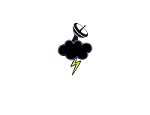
\includegraphics[width=9cm]{images/mobicharged.png} 
}
\author{Team Super Charged (No.33)
		\\ Nashit Mohammad - mohamn31
		\\ Eric Nguyen - nguyee13
		\\ Samuel De Haan - dehaas1
		\\ Eamon Earl - earle2
		\\ Mustafa Choueib - choueibm
}
    

\date{April, 2023}


\maketitle

\pagenumbering{roman}
\tableofcontents
\listoffigures
\listoftables

\vspace{20pt}


\newpage

\pagenumbering{arabic}

\section{Revision History}
\begin{center}
\begin{table}[H]
\caption{\bf Revision History}
    \begin{tabular}{p{2cm}p{3cm}p{2cm}p{6cm}}
    \hline
    \bf Author & \bf Date & \bf Version & \bf Description\\
    \hline
    Mustafa Choueib & April 4th, 2023 & Rev 0 & Created first draft of document\\
    \hline
    \end{tabular}
\end{table}
\end{center}


\section{Legal and Copyright Information}
This version of the MobiCharged software ("Software Product"), any documentation, or other forms of intellectual property are reserved by the Computing and Software Department of McMaster University, MobiCharged development team, and Mobilite Power Inc. The MobiCharged Software is protected by copyright laws and treaties, and other laws governing different forms of intellectual property. These are the Terms and Conditions governing the use of this Service and the agreement that operates between You and all Affiliates of this Software Product.

\subsection{Acceptance}
By installing, using, or accessing the Service You agree to be bound by these Terms and Conditions. If You fail to agree with ALL of the Terms and Conditions presented in this document, You may not use this Service.

\subsection{Prohibitions}
You are prohibited from:
\begin{itemize}
    \item Violating or attempting to violate the security of this Software Product.
    \item Violate any law, rule, or regulation while using this Software Product.
    \item Altering or attempting to alter, decompile, derive, or reverse engineer the Source code of this Software Product.
    \item Obtain or attempting to obtain unauthorized access to this Software Product.
    \item Using or attempting to use any device, software, or routine to interfere or attempt to interfere with the proper working of this Software Product. 
    \item Using or attempting to use any device, software, or routine to interfere, access, alter, or corrupt or attempt to interfere, access, alter, or corrupt any data in the database portion of this Software Product.
\end{itemize}
\subsection{Breach of Contract}
If You violate ANY of these rules, MobiCharged Affiliates may take action against You. This includes possible legal persecution, revoked access to this Software Product or any other Software Products provided by the MobiCharged development team. 

\subsection{Governing Law}
This Agreement is governed by the laws of the Province of Ontario.
\subsection{Exclusion of Liability}
TO THE FULLEST EXTENT PERMITTED BY LAW, ALL AFFILIATES OF THE MOBICHARGED SOFTWARE PRODUCT WILL NOT BE LIABLE IN CONNECTION WITH THIS CONTRACT FOR LOST PROFITS, BUSINESS OPPORTUNITIES, REPUTATION, DATA, OR ANY INDIRECT, INCIDENTAL, CONSEQUENTIAL, SPECIAL, OR PUNITIVE DAMAGES.
YOU AGREE THAT YOU ARE MAKING USE OF THIS SOFTWARE PRODUCT AT YOUR OWN RISK AND THAT IT IS PROVIDED ON AN "AS IS" BASIS. TO THE EXTENT PERMITTED BY LAW, WE EXCLUDE ALL EXPRESS OR IMPLIED WARRANTIES, TERMS AND CONDITIONS INCLUDING, BUT NOT LIMITED TO, IMPLIED WARRANTIES OF MERCHANTABILITY, FITNESS, AND NON-INFRINGEMENT.



\section{Introduction}
The MobiCharged Product consists of a Server-Client portion that autonomously runs simulations and stores data in a database, a machine learning black board that uses the data to be trained and provide optimal configurations, and a hardware system that aids in optimizing the algorithms in a real world environment. This User's guide contains an overview on the proper installation and use of the MobiCharged software and hardware product. 
\par
Note: The Server-Client portion is run as a background process in order to generate data with specific configurations (determined by the user) that will be used to train a specific model of the machine learner.

\section{Installation}
\subsection{Software Installation}
\subsubsection{Installing the Server}
As the Server is run on a remote host, the dependencies required will already be installed on that system. Only the Tkinter external package is required for the server configuration initializer, which can be installed by running "pip install tk" or "python.exe -m pip install tk" in the command line. Steps to connect to the remote host and launch the MobiCharged server are available in the Usage section of this document.
\begin{enumerate}
    \item Install any version of PuTTY (third party software to connect to remote hosts)
    \item Under "Host Name (or IP address)" enter "172.105.14.186" and keep the port as 22
    \item Provide a name and save the connection (to avoid entering the address each time)
    \item Enter the credentials provided by the MobiCharged team and launch the "launch\_server.bat" by using the "./launch\_server.bat" command in the console
    \item Ensure you are prompted with "MobiCharged server is now running...."
\end{enumerate}

\subsubsection{Installing the Client}
The client uses many different files and external dependencies in order to run correctly. Thus, on your machine you must ensure the following items are installed:
\begin{enumerate}
    \item MATLAB (versions other than R2023a may cause issues)
    \item MATLAB Engine (refer to: \href{https://www.mathworks.com/help/matlab/matlab_external/install-the-matlab-engine-for-python.html}{MATLAB Engine Instllation Guide})
    \item Download the MobiCharged client files
\end{enumerate}

\subsubsection{Installing the Machine Learner}
The Machine Learner uses the packages required to install the client and some additional external packages. The packages that must be installed on your machine are:
\begin{enumerate}
    \item Tkinter (can be installed by running "pip install tk" or "python.exe -m pip install tk" in the command line)
    \item Tenserflow (Refer to: \href{https://www.tensorflow.org/install/pip}{Tenserflow installation with pip})
    \item Firebase (Can be installed using "pip install python-firebase" in the command line. Refer to: \href{https://pypi.org/project/python-firebase/}{Firebase for Python} for more information)
    \item MATLAB (versions other than R2023a may cause issues)
    \item MATLAB Engine (refer to: \href{https://www.mathworks.com/help/matlab/matlab_external/install-the-matlab-engine-for-python.html}{MATLAB Engine Instllation Guide})
    \item The MobiCharged Machine Learner Black board package 
\end{enumerate}

\subsection{Hardware Installation}
The hardware system requires a small amount of setup/installation before it is ready to be used. To install the hardware system, you must do the following:
\begin{enumerate}
    \item Download the phasedarray.ino file from the MobiCharged Repository
    \item Download and Install the Arduino IDE (Refer to: \href{https://www.arduino.cc/en/software}{Arduino IDE})
    \item Have an Arduino system connected to your machine, and upload the phasedarray.ino file to the Arduino through the IDE
\end{enumerate}

\section{Usage}
\subsection{Using the Server-Client Application}
Note: The Server-Client Application does not need to be running to run the Machine Learner Black Board or use the hardware system. 
\subsubsection{Configuring the MobiCharged Server}
To configure the server prior to launch, you should locate your MobiCharged server files and run the mobicharged\_initializer.exe to start the initializer application. If you have trouble launching the initializer with the .exe file, it can also be run through the command line by navigating to the path of the mobicharged\_initializer.py file and using the command "python mobicharged\_initializer.py". 
\begin{figure}[H]
    \centering
    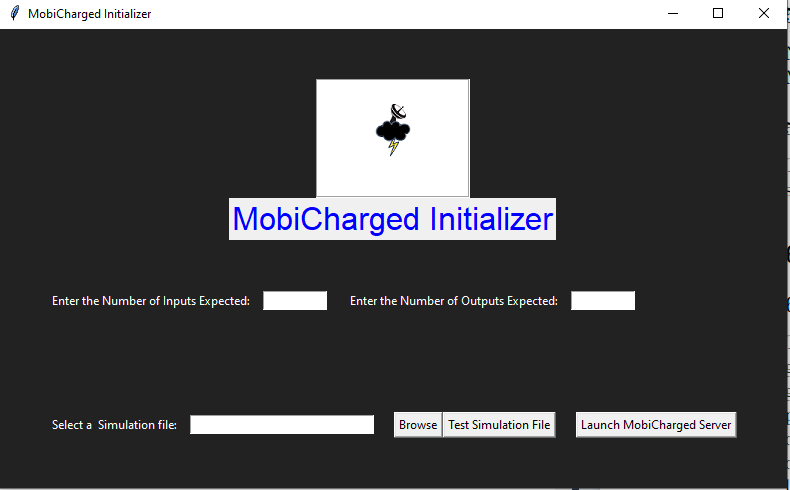
\includegraphics[width=12cm]{images/MobiCharged_initializer.PNG}
    \caption{MobiCharged Initializer}
    \label{fig:my_label}
\end{figure}

Once the initializer is open, begin filling out the input boxes with your desired specifications. Once you enter the number of inputs expected (first entry), more fields will be generated asking for specific ranges to be used in generating random input (for autonomous data generation). 
\begin{figure}[H]
    \centering
    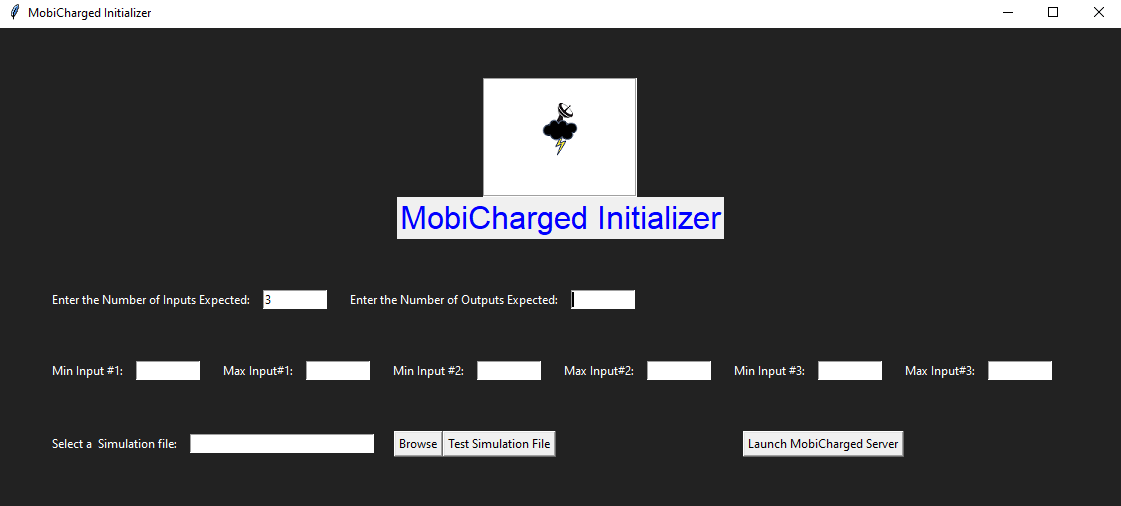
\includegraphics[width=12cm]{images/newinputfields.PNG}
    \caption{MobiCharged Initializer}
    \label{fig:my_label2}
\end{figure}
You will also be asked to select a specific MATLAB simulation file and run a quick test using the inputs provided to ensure that the desired configuration is compatible with the desired simulation file. Once all the fields have been filled and a MATLAB simulation file has been selected and tested (test must be successful, otherwise you will not be able to launch the server), press the "Launch MobiCharged Server" button to create a server with the given specifications.

\subsubsection{Starting the Configured Server}
To start the server that was just configured, open the third-party application PuTTY and connect to the remote host specified in the Installation section of this document. You will be prompted to enter a username and password, which authorized users should have received. Upon providing the correct credentials, a file named "launch\_server.bat" will exist providing all the specifications from the initializer. Use the command './launch\_server.bat" to start the server.
\begin{figure}[H]
    \centering
    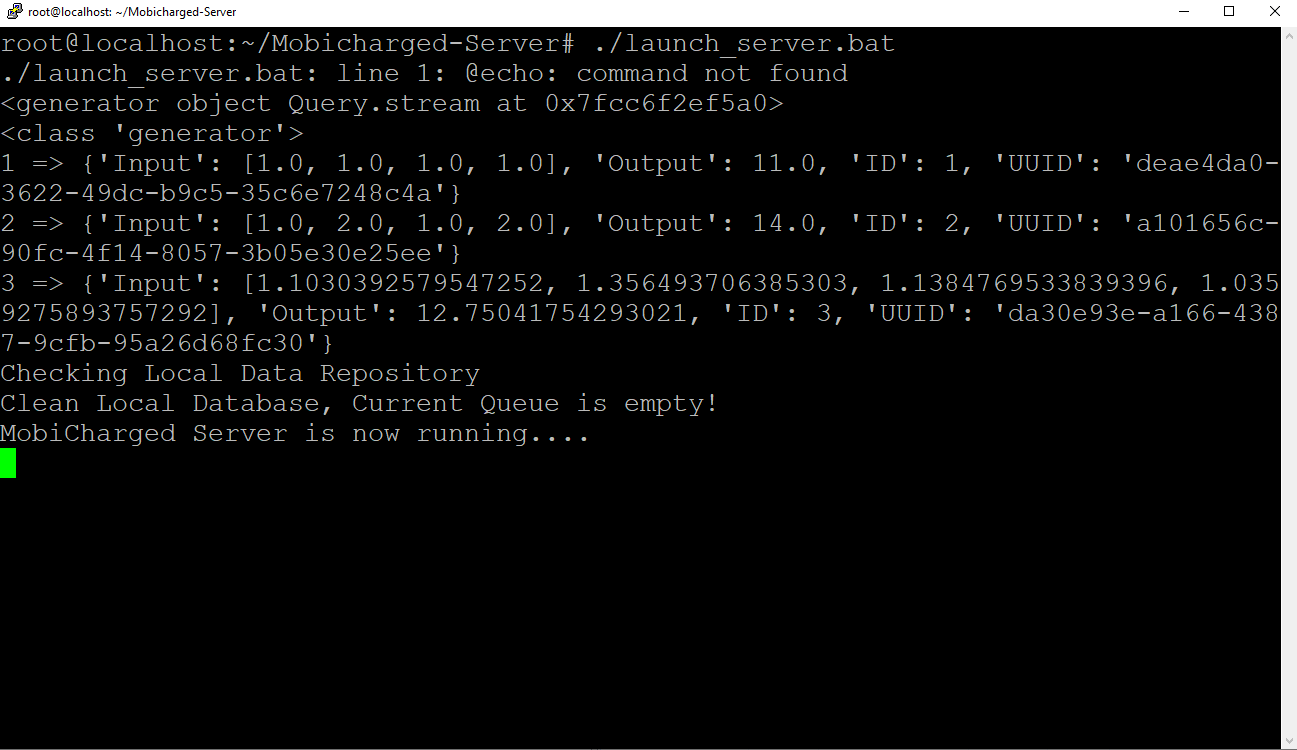
\includegraphics[width=12cm]{images/launchserver.PNG}
    \caption{Remote Host}
    \label{fig:my_label3}
\end{figure}

\subsubsection{Starting the Clients}
The clients can be run from any machine, given it was installed correctly. Thus, download the client files from the MobiCharged repository and run the "client\_controller.py" file using the command "python client\_controller.py". The simulation file the server is expecting will be displayed to the client, and the client will enter the path to a simulation file (same simulation file should be used to avoid conflict). From there, the client will request more input then it will begin the autonomous cycle with the server. 
\begin{figure}[H]
    \centering
    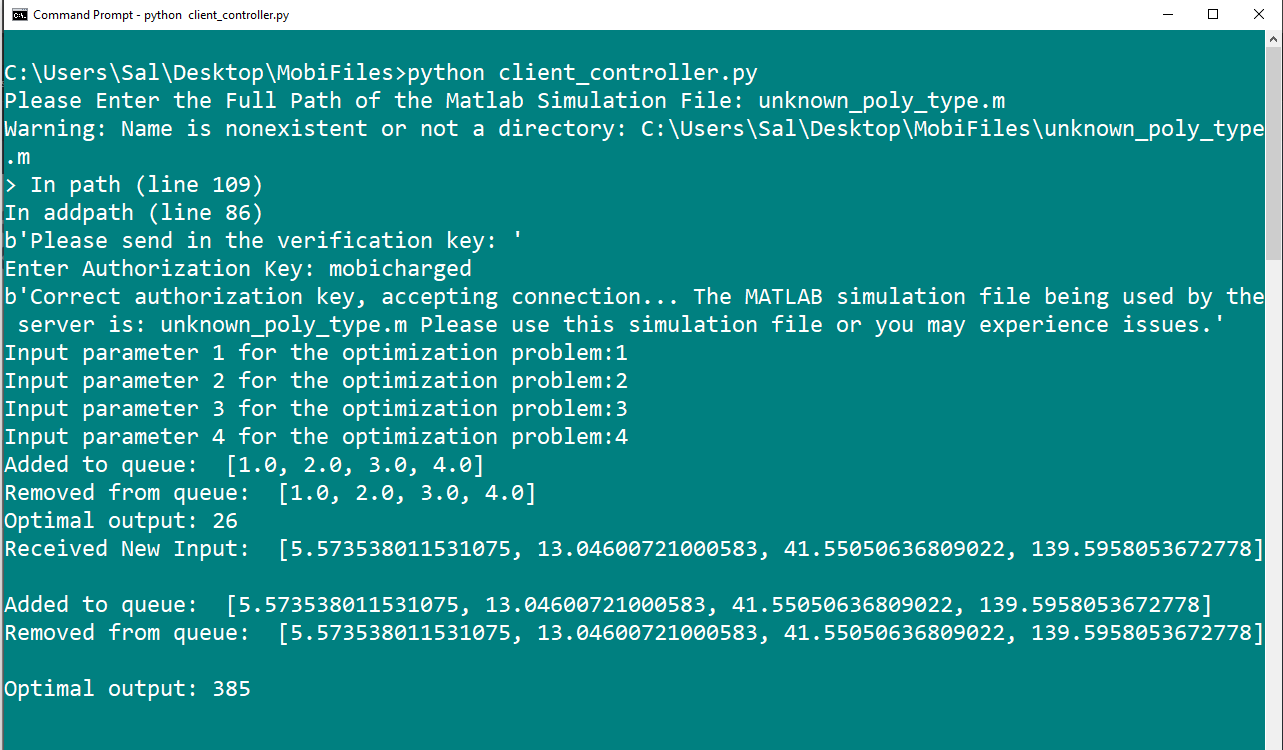
\includegraphics[width=12cm]{images/clientinteraction.PNG}
    \caption{Client Side Application}
    \label{fig:my_label4}
\end{figure}
\begin{figure}[H]
    \centering
    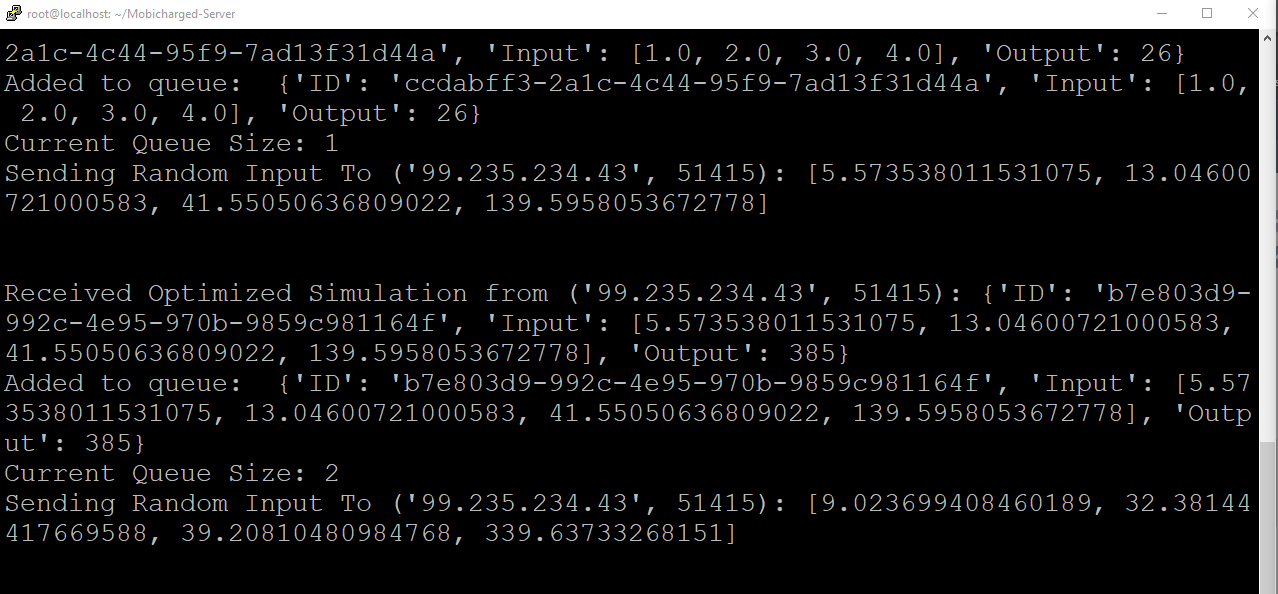
\includegraphics[width=12cm]{images/serverinteraction.PNG}
    \caption{Server Side Application}
    \label{fig:my_label5}
\end{figure}
The first input parameters are just initial random parameters, after this, the server and client should interact with each other and generate data without any user involvement. As you can see from figure 5, the Server will send back "Random Input" and the client will calculate optimal output for that input. This cycle will continue until stopped by the user.

\subsection{Using the Machine Learner Black Board}
To initialize the Machine Learning Blackboard system, we first want to run the src/reset.py script. This will ensure that the system state is correct and ready to be started anew. This script will ask you to confirm in the terminal with a "Y" that you wish to reset the system state. This should be done every time you want to rerun the Blackboard with a clean slate (without any current best model permeated and without any under-performing models being labeled invalid). 

From there, we would ask that you run the MLB\verb|_|GUI.py script. This will initialize the front end of the system. From there, you can click on the "ML Blackboard start" button. This will begin the process of pitting the models against each other. Note that the GUI will be mostly unresponsive until convergence. Upon convergence on a single best model, the GUI will present a graph representing its error progression throughout the run that yielded the model our "locally optimal" weights. We should also expect the first table to be populated with the iteration number, the winning model, the average absolute error, and so on. From there, you can click on the button that says "unknown\verb|_|poly\verb|_|type", and then on the subsequent button of the same name (this will have more options if we have multiple simulation files available to be tested against). From here, you will see a table render below the error graph, where you can input your data points you wish to predict on. For the time being, we are also computing the real outputs of these inputs and calculating the actual error to compare it to the expected error. 

This process can be repeated any number of times, and the "ML Blackboard start" button can be clicked again as well. Expect subsequent training to be faster than the initial one, and that once converged naturally (not stopped prematurely), the ML Blackboard process will have found a sole victor and the other models that were initially there will not be trained on. If you wish to train on them again, you can run the reset.py script as previously discussed, though this will also reset our prior knowledge of our best contender, or if you want you could manually move the models from src/invalid\verb|_|models to src/valid\verb|_|models to keep the knowledge of our best model. Feel free to close and rerun the GUI at any point in the process.

The Blackboard has been preloaded with two naive models, for the sake of exemplifying the product in a controlled manner.


\subsection{Using the Hardware System}
To use the hardware system, start by connecting the array power source to a 120V supply. Assuming installation was done correctly, once connected to a 120V supply, turn the power switch on to provide power to the array. Once the hardware system is powered on, use tweezers to insert the desired particle for levitation. The particle inserted should be levitating and can be controlled by closing the "up switch" or "down switch" to move the particle vertically, or close the "reset switch" to return the particle to the centre. 

\section{Troubleshooting}
\subsection{Server Initializer Errors}
\textbf{Error: MATLAB Simulation Failed}
\newline
This error means that the selected MATLAB simulation file is not compatible with the specified parameters. The user must ensure that the specified parameters is compatible with the MATLAB simulation file and run the test again to be able to launch the server.


\subsection{Server Errors}
Server sided errors are displayed in the console of the remote host. Here is a list of potential errors:
\newline
\newline
\textbf{Error: Failed to Launch Server}
\newline
This error can occur for many reasons; manual modifications to the local database, invalid specifications, corrupted launch\_server.bat file. The solution to this would be to reconfigure the server, and launch it.



\subsection{Client Errors}
Client sided errors are displayed in the console of the users machine. Here is a list of potential errors:
\newline
\newline

\textbf{Error: MATLAB Engine Error}
\newline
If you see this error, either the specified inputs or the chosen MATLAB simulation files are not compatible, thus, cannot produce a result from MATLAB Engine.
\newline
\newline
\textbf{Error: Connection Refused Error}
\newline
If you see this error, that means the client could not connect to the server. This is typically because the server is not launched and the client is trying to connect.

\subsection{Machine Learner Errors}

Ensure that you have run reset.py and confirmed the reset in the terminal before running the main loop.

MOST IMPORTANT TROUBLESHOOT: Ensure that you are running the files from WITHIN the MobiCharged folder, such that MobiCharged is our parent folder and we are in the same directory as the src folder. We were having issues with absolute pathing, and noted that if you run it with src as your root file you will encounter pathing errors. This will be remedied and standardized at launch.

A possible pseudo-error state is that the Blackboard is taking an eerily long time to converge. And as such the option to predict does not open for some time. With the two given models, and the likely small database size we will be providing for marking, you should expect convergence within 5 minutes. If this does not occur, check the terminal. If the training errors being reported there are infinite or NaN, then our input data is ill-defined and it is unlikely that the Blackboard will converge. If this happens, reach out to us and we will go about re-generating some data that plays nicer with our naive machine learning models.

It is unlikely that we will be generating great deals of data, so do not expect high accuracy from these models. If, however, we do have a very full database, there is a possibility of a memory error occuring, in which case you can once again reach out to us and we will slash down our database, as I think this is easier than asking you to do something on your end.


\section{Frequently Asked Questions and Answers}
\textbf{Question:} What can be levitated?
\newline
\textbf{Answer:} An object whose density is less than ~4g/cm (cubed). This includes liquids and solids. Objects of uniform shape (spheres) are more stable.
\newline
\newline
\textbf{Question:} How long can the array run?
\newline
\textbf{Answer:} The array can run as long as any of the electrical components remain at a reasonable temperature. Results have show this to be greater than 2 hours.
\newline
\newline
\textbf{Question:} How many clients can connect to the server?
\newline
\textbf{Answer:} There is no limitation on the number of clients that connect to a server. The server was tested with over 25 clients connected at once and experienced little to no loss in performance.
\newline
\newline
\textbf{Question:} Can I run more than one client on a machine?
\newline
\textbf{Answer:} Yes, you can run an unlimited amount of clients on one machine, or many machines.
\newline
\newline
\textbf{Question:} What happens if the server or client are interrupted during data transmissions?
\newline
\textbf{Answer:} The Server-Client application was designed to prevent any loss or corruption in data, thus, should be fine once either the client or server are restored.

\section*{References}
[1] Hartley, C. (2023, February 18). User agreement template. TermsFeed. Retrieved April 5, 2023, from https://www.termsfeed.com/blog/sample-user-agreement-template/ 
\newline
Any other sources refer to documentation provided by Mobilite-Power.




\end{document}

